\documentclass[11pt]{article}
\usepackage[landscape,margin=1.4cm]{geometry}
\usepackage{tikz}
\usepackage{amsmath}
\usepackage{booktabs}
\usepackage{array}
\usepackage{xcolor}
\usetikzlibrary{positioning,arrows.meta,shapes.geometric,shapes.misc,calc}

% ---- palette (matches bank_fsm.excalidraw) ----
\definecolor{cStart}{HTML}{FED7AA}\definecolor{cStartS}{HTML}{C2410C}
\definecolor{cDec}{HTML}{FEF3C7}\definecolor{cDecS}{HTML}{B45309}
\definecolor{cPre}{HTML}{93C5FD}\definecolor{cAct}{HTML}{60A5FA}\definecolor{cCas}{HTML}{3B82F6}
\definecolor{cEnd}{HTML}{A7F3D0}\definecolor{cEndS}{HTML}{047857}
\definecolor{cRef}{HTML}{DDD6FE}\definecolor{cRefS}{HTML}{6D28D9}
\definecolor{cArb}{HTML}{DBEAFE}\definecolor{cArbS}{HTML}{1E40AF}
\definecolor{cNS}{HTML}{1E3A5F}\definecolor{cSlate}{HTML}{64748B}
\definecolor{cWarn}{HTML}{FEE2E2}\definecolor{cWarnS}{HTML}{DC2626}

\tikzset{
  state/.style={rounded corners=4pt,draw=cNS,line width=1pt,minimum width=2.5cm,minimum height=1.1cm,align=center,font=\small\bfseries},
  term/.style={ellipse,draw,line width=1pt,minimum width=2.4cm,minimum height=1.1cm,align=center,font=\small\bfseries},
  dec/.style={diamond,aspect=1.7,draw=cDecS,fill=cDec,line width=1pt,align=center,font=\small,inner sep=1pt},
  edge/.style={-{Stealth[length=6pt]},line width=1pt,draw=cNS},
  cedge/.style={-{Stealth[length=6pt]},line width=1pt,draw=cDecS},
  elbl/.style={font=\scriptsize,color=cSlate},
  clbl/.style={font=\scriptsize\bfseries},
}

\setlength{\parindent}{0pt}
\begin{document}

{\LARGE\bfseries\color{cArbS} Per-Bank Request FSM \;--\; RMC DDR5 Scheduler}\\[2pt]
{\small\color{cSlate} One bank shown; \texttt{N\_BANKS} copies run independently, merged by the weight arbiter (1 cmd / 2\,tCK). Timing = \texttt{b4800} bin (tCK 0.4167\,ns). Companion to \texttt{scheduler\_bank\_fsm.md} / \texttt{scheduler\_staged\_logic.md}.}\\[10pt]

% ======================= FSM =======================
\begin{center}
\resizebox{!}{4.3cm}{%
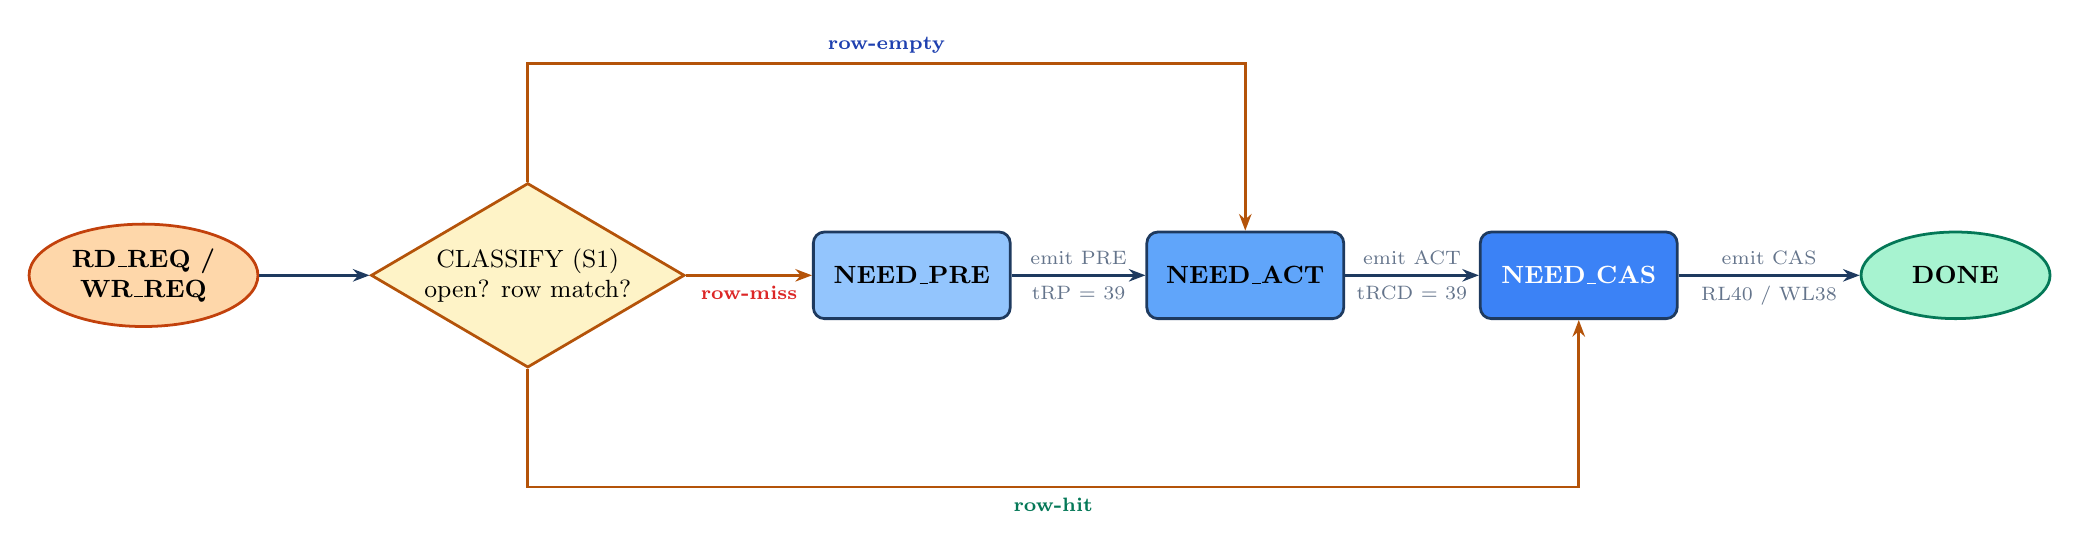
\begin{tikzpicture}[node distance=1.5cm]
  \node[term,fill=cStart,draw=cStartS] (arr) {RD\_REQ /\\WR\_REQ};
  \node[dec,right=1.4cm of arr] (cls) {CLASSIFY (S1)\\open? row match?};
  \node[state,fill=cPre,right=1.6cm of cls] (pre) {NEED\_PRE};
  \node[state,fill=cAct,right=1.7cm of pre] (act) {NEED\_ACT};
  \node[state,fill=cCas,text=white,right=1.7cm of act] (cas) {NEED\_CAS};
  \node[term,fill=cEnd,draw=cEndS,right=2.3cm of cas] (done) {DONE};

  \draw[edge] (arr) -- (cls);
  \draw[cedge] (cls) -- node[clbl,color=cWarnS,below]{row-miss} (pre);
  \draw[cedge] (cls.north) -- ++(0,1.5) -| node[clbl,color=cArbS,pos=0.25,above]{row-empty} (act.north);
  \draw[cedge] (cls.south) -- ++(0,-1.5) -| node[clbl,color=cEndS,pos=0.25,below]{row-hit} (cas.south);

  \draw[edge] (pre) -- node[elbl,above]{emit PRE} node[elbl,below]{tRP = 39} (act);
  \draw[edge] (act) -- node[elbl,above]{emit ACT} node[elbl,below]{tRCD = 39} (cas);
  \draw[edge] (cas) -- node[elbl,above]{emit CAS} node[elbl,below]{RL40 / WL38} (done);
\end{tikzpicture}}
\end{center}

\vspace{2pt}
{\small Read and write share the FSM; only the CAS flavour (\texttt{CAS\_RD}/\texttt{CAS\_WR}) and the tail timing differ (write adds \texttt{tWR} recovery before PRE). \textbf{No marching token} --- every \texttt{NEED\_*} slot nominates in parallel; the arbiter emits one.}

\vspace{6pt}
% ======================= two-column: arbiter + tables =======================
\begin{minipage}[t]{0.46\textwidth}
{\large\bfseries\color{cArbS} Weight arbiter --- emission control}\\[6pt]
\resizebox{\textwidth}{!}{%
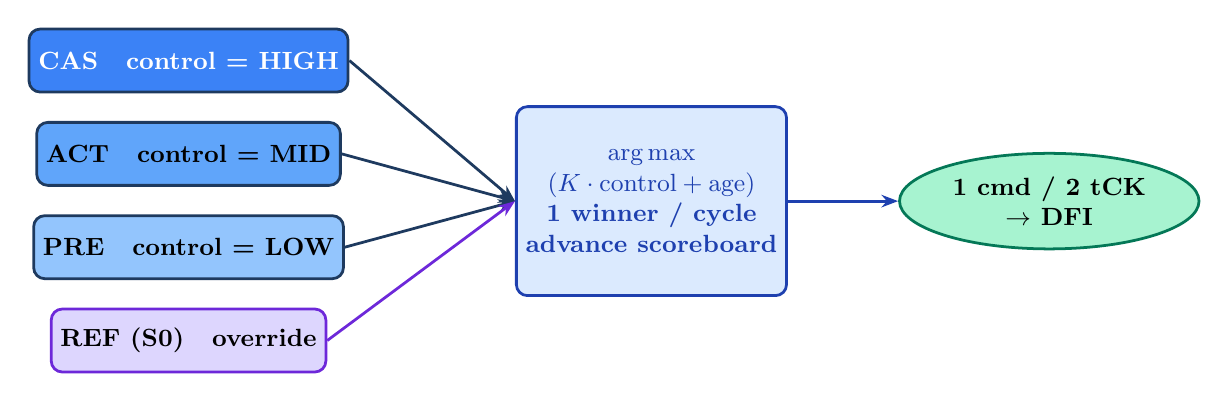
\begin{tikzpicture}[node distance=0.35cm]
  \node[state,fill=cCas,text=white,minimum width=3.2cm,minimum height=0.8cm] (lc) {CAS \; control = HIGH};
  \node[state,fill=cAct,minimum width=3.2cm,minimum height=0.8cm,below=of lc] (la) {ACT \; control = MID};
  \node[state,fill=cPre,minimum width=3.2cm,minimum height=0.8cm,below=of la] (lp) {PRE \; control = LOW};
  \node[state,fill=cRef,draw=cRefS,minimum width=3.2cm,minimum height=0.8cm,below=of lp] (lr) {REF (S0) \; override};
  \node[state,fill=cArb,draw=cArbS,text=cArbS,minimum width=3.4cm,minimum height=2.4cm,right=2.2cm of la.east,yshift=-0.6cm,align=center] (arb) {$\arg\max$\\$(K\cdot\mathrm{control}+\mathrm{age})$\\1 winner / cycle\\advance scoreboard};
  \node[term,fill=cEnd,draw=cEndS,right=1.4cm of arb,minimum width=2.6cm] (out) {1 cmd / 2 tCK\\$\rightarrow$ DFI};
  \draw[edge] (lc.east) -- (arb.west);
  \draw[edge] (la.east) -- (arb.west);
  \draw[edge] (lp.east) -- (arb.west);
  \draw[edge,draw=cRefS] (lr.east) -- (arb.west);
  \draw[edge,draw=cArbS] (arb) -- (out);
\end{tikzpicture}}
\\[8pt]
{\footnotesize \textbf{Aging:} \texttt{age[lane] += 1} every waiting cycle (incl.\ timing-blocked); \texttt{= 0} on win. Starved lane climbs until it preempts --- bounded starvation.}\\[6pt]
\fcolorbox{cWarnS}{cWarn}{\parbox{0.95\textwidth}{\footnotesize\color{cWarnS}\textbf{$\triangle$ Scaling caveat (weights pass).} Age ticks \emph{every} waiting cycle, so without the $K$ scale it swamps the fixed control weight and the arbiter degenerates to oldest-first (loses CAS-first). $K$, control values, and \texttt{AGE\_MAX} = one joint knob-set.}}
\end{minipage}\hfill
\begin{minipage}[t]{0.5\textwidth}
{\large\bfseries\color{cArbS} Classify --- the fork}\\[4pt]
{\footnotesize
\begin{tabular}{@{}l l l l@{}}
\toprule
\textbf{bank state} & \textbf{case} & \textbf{chain} & \textbf{work\_state}\\
\midrule
closed / idle & row-empty & \texttt{ACT$\to$CAS} & NEED\_ACT\\
open, \texttt{row==R} & row-hit & \texttt{CAS} & NEED\_CAS\\
open, \texttt{row!=R} & row-miss & \texttt{PRE$\to$ACT$\to$CAS} & NEED\_PRE\\
\bottomrule
\end{tabular}}
\\[10pt]
{\large\bfseries\color{cArbS} Latency chains (tCK, b4800)}\\[4pt]
{\footnotesize
\begin{tabular}{@{}l l r@{}}
\toprule
\textbf{case} & \textbf{chain} & \textbf{first data}\\
\midrule
row-hit \emph{(best)}, rd & \texttt{CAS} & RL = 40\\
row-hit, wr & \texttt{CAS} & WL = 38\\
row-empty, rd & \texttt{ACT$\to$CAS} & 39+40 = 79\\
row-miss \emph{(worst)}, rd & \texttt{PRE$\to$ACT$\to$CAS} & 39+39+40 = \textbf{118}\\
\quad + full burst & \quad + BL/2 & +8 = \textbf{126}\\
row-miss + refresh & \texttt{...REF...$\to$PRE$\to$ACT$\to$CAS} & +tRFC = +708\\
write tail $\to$ PRE & \texttt{CAS\_WR $\to$ ... $\to$ PRE} & WL+BL2+tWR = 118\\
R$\to$W turnaround & \texttt{CAS\_RD$\to$CAS\_WR} & tRTW = 12\\
W$\to$R turnaround & \texttt{CAS\_WR$\to$CAS\_RD} & +tWTR\_L = 70\\
\bottomrule
\end{tabular}}
\\[8pt]
{\footnotesize $L_{\text{miss}}=126$\,tCK, service $=$ BL/2 $=8$\,tCK/burst $\Rightarrow$ latency floor $N=L_{\text{miss}}/8\approx16$ in-flight reads to hide one row-miss. Buffer depth = 64 (margin). See \texttt{staged\_logic} \S0.}\\[6pt]
{\footnotesize\color{cSlate} \texttt{N\_BANKS} FSMs run in parallel; cross-bank \texttt{tCCD\_L / tRRD\_L / tFAW / DQ} apply at the arbiter, not inside a bank. Paths $\neq$ emissions: CA bus is 1 cmd / 2\,tCK.}
\end{minipage}

\end{document}
